Following the initial data integration, this section performs a detailed Exploratory Data Analysis (EDA) on the merged Land Cover dataset (\texttt{landcover\_combined.geojson}) to assess its structure, identify redundant features, and prepare the complex classification codes for modeling.

\subsection{Data Structure and Integrity}

The merged Land Cover GeoDataFrame (\texttt{landcover\_gdf}) was loaded and inspected for structural consistency.

\begin{itemize}
    \item \textbf{Data Counts:} The total number of unique features and the distinct values for the primary classification columns—$\texttt{lcccode}$ (Land Cover Classification Code) and $\texttt{gridcode}$—were tallied.
    \item \textbf{Redundancy Check:} An inspection for rows with duplicated $\texttt{id}$ values was performed. Although duplicates were found, the difference in associated geometry or attributes suggested they were not true feature duplicates, and the $\texttt{id}$ column was deemed non-essential for the model and slated for removal.
    \item \textbf{Missing Values:} A check across all columns confirmed the absence of any null or NaN values, indicating a complete and clean dataset structure following the initial GeoJSON conversion.
\end{itemize}

\textbf{Relationship between Classification Codes}
A key analysis focused on the relationship between $\texttt{gridcode}$ and $\texttt{lcccode}$. By checking unique pairs of these two columns, it was determined that they possess a one-to-one relationship. Consequently, $\texttt{gridcode}$ was identified as a redundant column that provides no additional information and is recommended for dropping during preprocessing.

 

\subsection{Initial Visualization and Area Analysis}

% \begin{figure} [H]
%     \centering
%     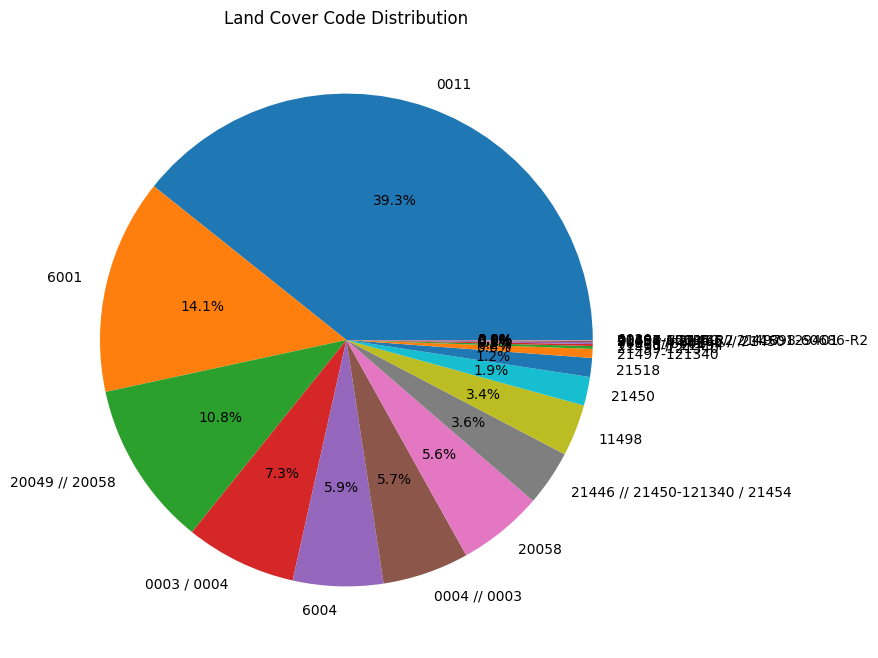
\includegraphics[width=0.8\textwidth]{images/LandCover/pie chart land cover distribution.png}
%     \caption{Pie chart illustrating the proportional distribution of Land Cover Codes ($\texttt{lcccode}$) across the combined study area.}
%     \label{fig:lcccode\_pie}
% \end{figure}

The distribution of land cover types was visualized to understand the regional composition:
\begin{itemize}    
    \item \textbf{Distribution Map:} The Land Cover Map was plotted, coloring polygons based on their $\texttt{lcccode}$ to visualize the spatial arrangement of classes.
    \begin{figure} [H]
    \centering
    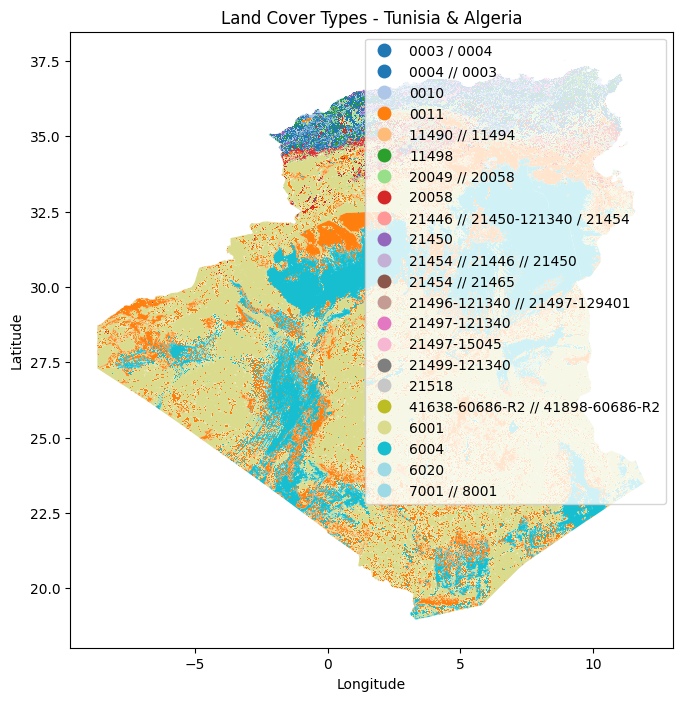
\includegraphics[width=0.5\textwidth]{images/LandCover/Land Cover Types - Algeria and Tunisia Merged.png}
    \caption{Geospatial visualization of the merged Land Cover Map, colored by the specific Land Cover Classification Code ($\texttt{lcccode}$).}%
    \label{fig:landcover_map}
\end{figure}

    % \item \textbf{Proportional Distribution:} A pie chart displayed the percentage distribution of each unique $\texttt{lcccode}$.
    \item \textbf{Area Analysis:} The geometric area of each polygon was calculated \\ ($\texttt{landcover\_gdf['area'] = \ldots geometry.area}$). A bar plot was generated showing the Total Area by Land Cover Code.


    \begin{figure} [H]
        \centering
        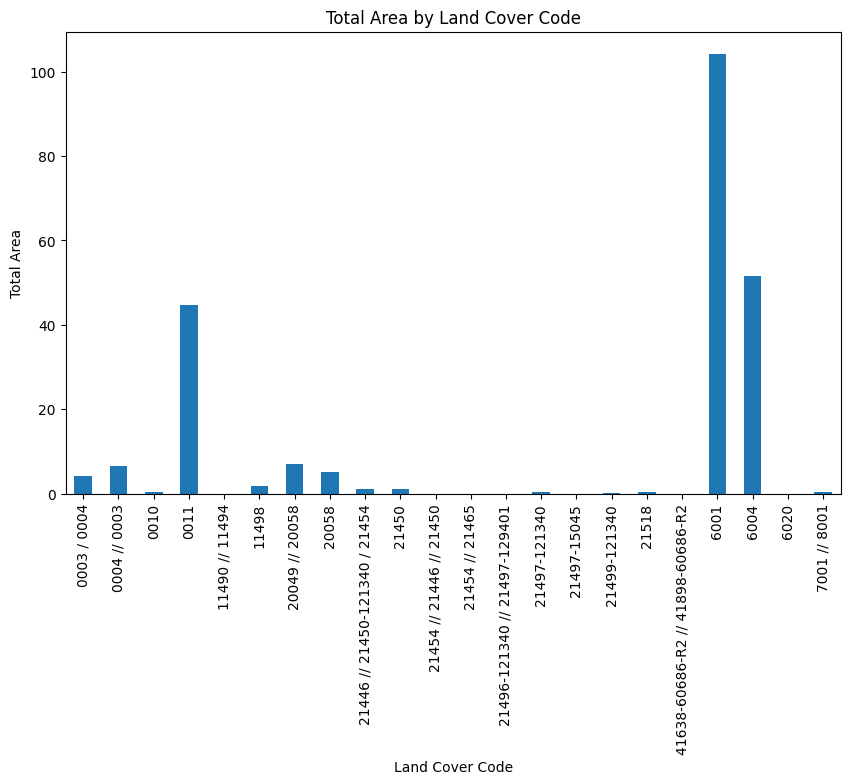
\includegraphics[width=0.6\textwidth]{images/LandCover/total area by lcc code bar chart.png}
        \caption{Total aggregated area (in square degrees) covered by each Land Cover Code in the combined dataset.}%
        \label{fig:lcccode_area}
    \end{figure}
\end{itemize}

 

% \subsection{Classification Code Harmonization}

% The raw $\texttt{lcccode}$ column contains complex codes (e.g., \texttt{7001 // 8001}) which represent mixed, uncertain, or transitional land cover types. The separator (\texttt{//}) indicates a mixture between the two classes (e.g., Shrubland and Bare/Sparse vegetation). To handle this complexity for machine learning, the following steps were taken:

% \textbf{Legend Integration}
% The official legend files (\texttt{globcover\_LCCS\_legend\_africa.xls} and \texttt{globcover\_legend.xls}) were loaded to establish a mapping between the numeric codes and descriptive labels.

% \begin{itemize}
%     \item The $\texttt{LCCCode}$ was mapped to its descriptive label ($\texttt{LCCOwnLabel}$) using a dictionary.
%     \item This process identified that certain codes were designated as ``Error'' in the $\texttt{LC}$ column of the legend, yet represented valid land cover types in the $\texttt{LCCOwnLabel}$ column (e.g., ``Closed forest''). This confirmed that these codes should be retained and mapped correctly.
% \end{itemize}

% \textbf{High-Level Mapping}
% Given the 22 unique $\texttt{lcccode}$ values in the dataset, a high-level, simplified mapping was created to aggregate these codes into fundamental categories (e.g., ``Forests,'' ``Bare lands,'' ``Croplands,'' ``Vegetation,'' etc.). 
% This step is crucial for reducing the complexity of the model's fire prediction.